\chapter{TLS echoservice}

The web service presented in the previous chapter has the mayor drawback that the communication between the two endpoints is unsecure.
Due to that reason the service  shall be extended by an additional layer called TLS (Transport Layer Security) to provide a certain degree of securtity on \task{Grid-level <-- explain that}.
%
In general the internet security is often subdivided into the following categories:~\cite{TANNENBAUM_2001}\task{verfiy citation}
\begin{itemize}
	\item \textbf{Confidentiality} --- Protection of the data against passiv attacks (such as publicise message content)
	
	\item \textbf{Authentication} --- Verification of the Authenticity  of the communications partner.

	\item \textbf{Integrity} --- Protection against interception and manipulation,replay,insertion, etc.  of a message.

	\item \textbf{Non-repudiation} --- Preventing the sender to repudiate the message transmitted by him.

	\item \textbf{Access control} --- Restrict the access to ressources.

	\item \textbf{Availability} --- Ensure a system is always usable which is challenged by several attacks.

\end{itemize}
%1-21   Gebräuchliche Dienste
%     Identifizierung           Vermerk
%     Berechtigung              Zugriff
%     Lizenz/Zertifizierung     Gültigkeitsprüfung
%     Unterschrift              Zeitpunkt des Auftretens
%     Bezeugung                 Abstimmung
%     Übereinstimmung           Eigentum
%     Zuverlässigkeit           Registrierung
%     Quittungen                Genehmigung/Verbot
%     Bestätigung des Ursprungs Privatsphäre
%
% Nach Sicherheit in verteilten Systemen, ITM Lübeck
The TLS to be introduced provides: Confidentiality, authentication, integrity, non-repudiation and access control.
It is introduced after the TCP layer. 
%
Before presenting the implementation of the new secure echo service the basic concept of a secure certifcate based connection shall be explained. Its not the goal to give an exact technical desciption but to give a first inside what is required to ensure the security of the layer.

% It is recommand to satifiy as much categories as possible. 
%authentication , confidentiality and integrity protection of TCP-based communication --- non-repudiation due to private key, access control to our service.


\section{Transport Layer Security}


The TLS is a protocol which provides a secure connection between two endpoints. It is located directly upon the TCP/IP layers and uses typically an asymmetric encryption to establish the connection (alternatively a symmetric pre-shared key may be used). After the communication has successfully established, both participants are switching to another encryption method which is based on a new negotiated symmetric key.
%    1. Peer negotiation for algorithm support
%    2. Key exchange and authentication
%    3. Symmetric cipher encryption and message authentication   - from wikipedia
%
%
Symmetric and asymmetric encryption are the two main classes of cryptography algorithms.
In case of a symmetric encryption both participants are holding the same secret key. 
Symmetric encryption can be ranked as being very secure but its downside is the key distribution which is very difficult in practice. 
Ideally the secret key is transmitted over a secure channel which is either a complete diffrent medium (i.e. a letter) or an channel encrypted with another secret key.
Asymmetric encryption follows a diffrent functional principle. While the symmetric encryption utilise one shared secret, the asymmetric ecryption is based on two keys: a private key and public key. As the names imply the private key is kept secret and never shared while the public key is available for everyone. Messages encrypted with the public key can only be decrypted with the private key and the other way round, messages encrypted with the private key can only be decrypted with the public key. The figure~\ref{fig:asymmetric_encryption} illustrates the circumstances of the case.\\
\begin{figure}[htb]
	\centering%epstopdf async.eps
	\subfloat[Texttext\label{fig:cgd}]
		{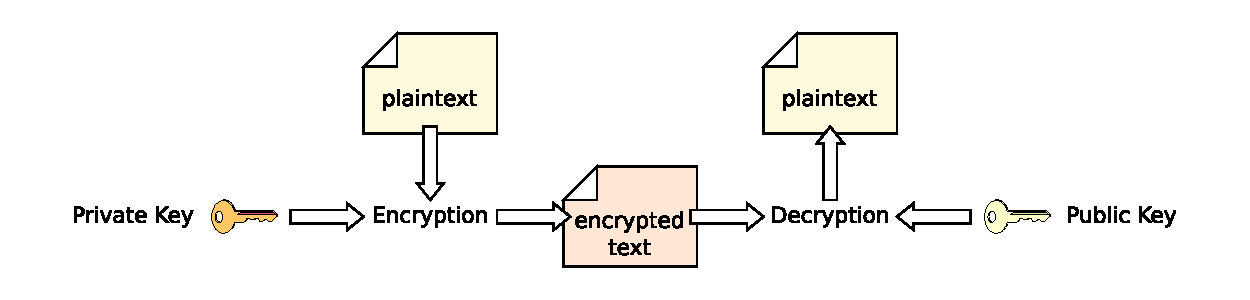
\includegraphics[width=12cm]{tex_tls_echoservice/async.pdf}}\\
	\subfloat[Texttext\label{fig:cgd}]
		{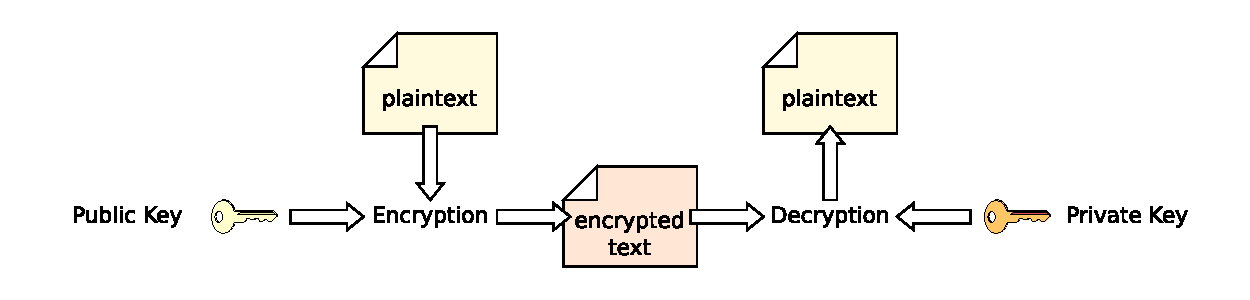
\includegraphics[width=12cm]{tex_tls_echoservice/async2.pdf}}
	\label{fig:asymmetric_encryption}
	\mycaption{specific}{general}
\end{figure}


At startup of the communication process A (Alice) who desires a secure connection transmits her public key to B (Bob).
Bob is now able to encrypt the messages such that only A is able to decrypt them.
That way confidentiality and integrity of messages are easily realised.
Non-repudiation, authentication and due to that access control are not given because the identity of Alice is not proven.
In order to be able to check identities so called certificates have been introduced.
Certificates render the possibility to check the identity of its owner. They are signed by a certificate authority (CA) which's identity can be resolved to another CA or is  pre-configured to be trusted.
A certificate is composed of its owner's public key, his identity, the name of the signing CA and a signiture which is a hash-value of the certificate encrypted with the private key of the CA. 
That way the CA confirms the identity of the certificate owner. 
To obtain a certificate a request has to be submitted to a CA which verifies the identity of the requesting person and signs it, if it comes to the result that the authenticity is valid. Figure~\ref{fig:certificate_request} shows the procedure to gain a certificate.
\begin{figure}[htb]
	\centering%epstopdf certificates.eps
 	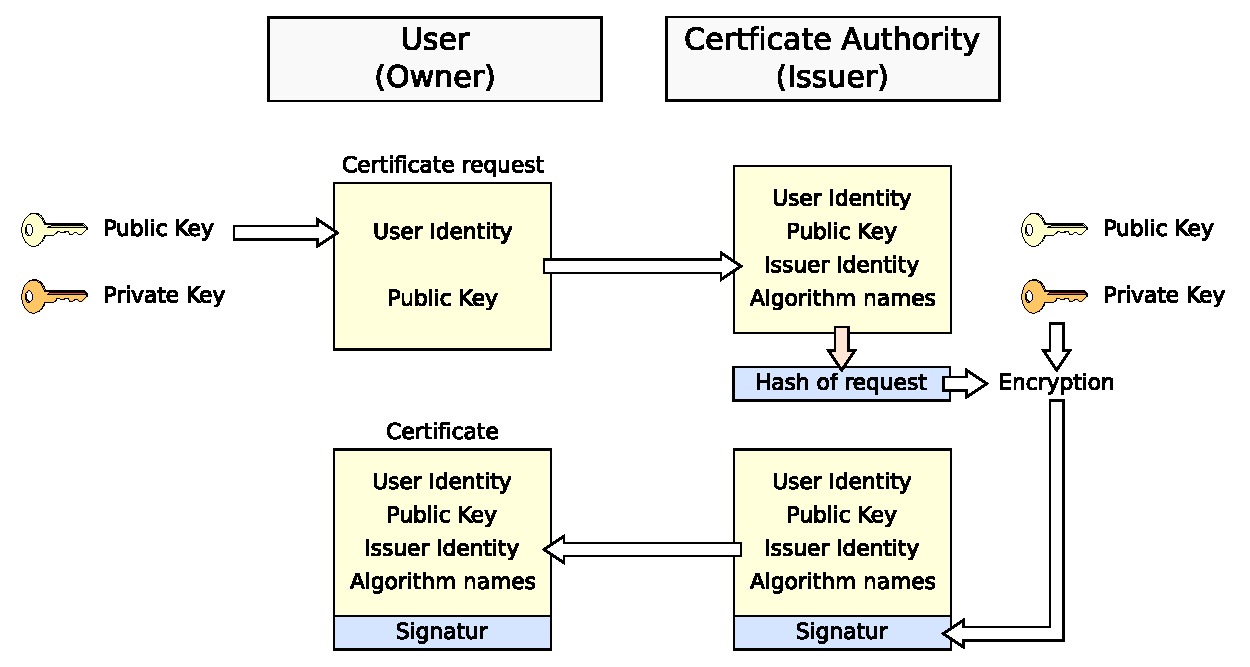
\includegraphics[width=13cm]{tex_tls_echoservice/certificates.pdf}
	\mycaption{specific}{general}
	\label{fig:certificate_request}
\end{figure}
Figure~\ref{fig:verification_of_certificates} shows a usecase where Alice wants to resolve the identity of Bob. Alice submitts her request to Bob along with a challange consisting of a random number $n$. Bob encrypts the number with his private key and returns it together with his certificate. With the usage of the public key, Alice is able to decrypt the challange which implies that, if the certificate is to be trusted, the identity of Bob is to be trusted. Unfortunately Alice is unable to verify the certificate because it is signed by an unknown CA called CA 1. She establishes the connection to CA 1 in order to resolve the identity of that certificate authority. Again Alice sends a challenge --- this time to the certificate authority CA 1. CA 1 encrypts the challange with its private key and submits the result along with its certificate. Again Alice validates the certificate sucessfully. 
The certificate was signed by a CA called CA 2 which she is able to locate as a pre-configured certificate. Due to the reason she trusts CA 2, she can trust CA 1 and finally Bob. 

\begin{figure}[htb]
	\centering%epstopdf verification.eps 
	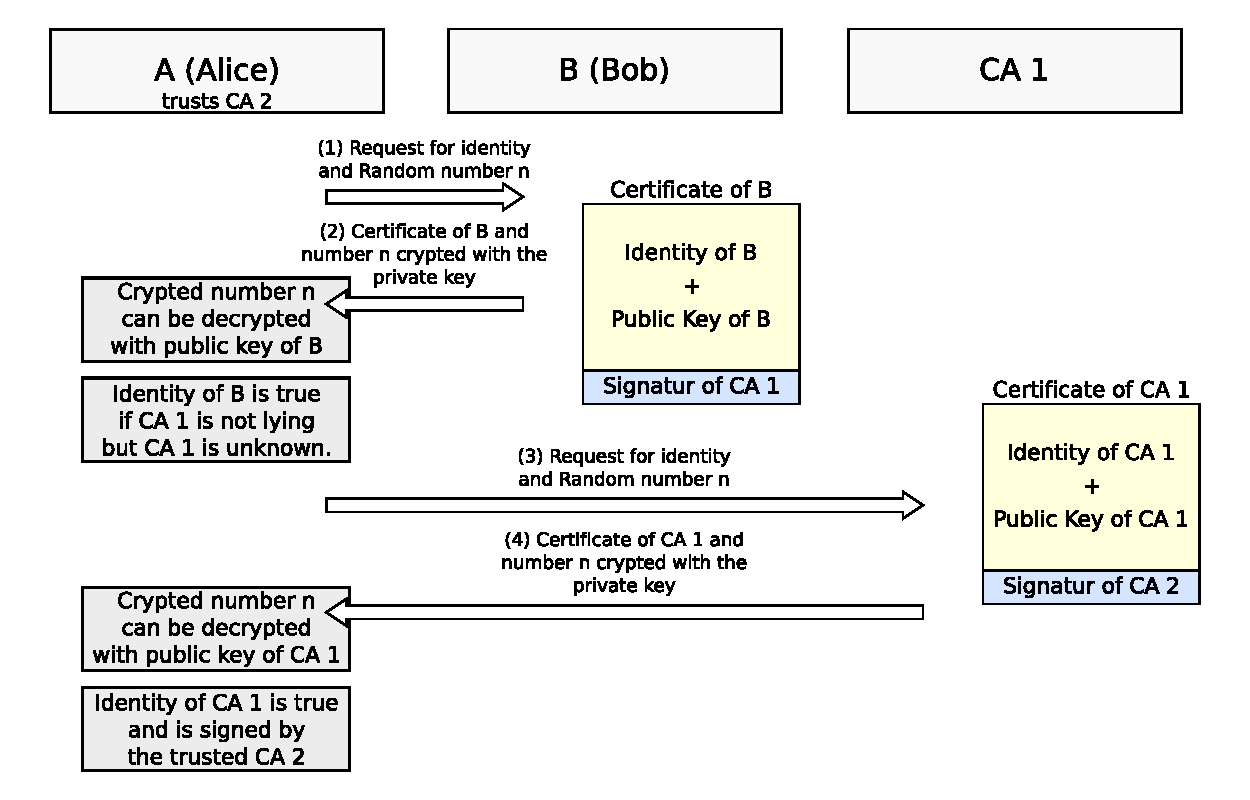
\includegraphics[width=13cm]{tex_tls_echoservice/verification.pdf}
	\mycaption{specific}{general}
	\label{fig:verification_of_certificates}
\end{figure}



The advantages of certificates are
o easy scalable to a larger set of users
o VOMs are realisable
o Infrastructure is given and easily to maintain
o In general the pre-configured organistion take money to sign certifcates, but they can also be created locally.



TLS also supports the more secure bilateral connection mode (typically used in enterprise applications), in which both ends of the "conversation" can be ensured with whom they are communicating




o What do we need to get a service running
clientCA   - Authority guarantee for identity
clientCERT - Certificate given
clientKEY  - Secret key of the client to read messages, encrypted by the public key in the certificate!

serverCA   - Authority guarantee for cert. CA is known by the server. If not, the encrypted cert can be read be its CA.
serverCERT - Certificate given by the CA. Contains a snippet which can be read by the Public key of the CA.
serverKEY  - Secret key of the client to read messages, encrypted by the public key in the certificate!


Server has got have:
Its  serverCERT serverKEY and some kind of root CA knowing the client
Client has got to have
Its  clientCERT clientKEY and some kind of root CA knowing the server













%The first two goals can be reached by encrypting the channel/connection between client and server. An approach 
%sich bewähren / behaupten
%which stand the test of time is to introduce a TLS (Transport Layer Security) also known as SSL (Secure Sockets Layer).
%Authenticity, Confidentiality, Integrity
%The client wants to reassure himself to send his vulnerable data only to the server who can prove its correct identity.
%Furthermore a prove of authenticity is needed. % Sich versichern, dass das Gegenüber der ist, für welchen er sich ausgibt
%It .... does fancy stuff ...
%
%
%Authorization:  The server on the other side takes an interest in limitate its ressources to a close circle of users. Above all no %foreign clients shall be able to use the services.\\


\clearpage
\section{Service}

One can add the TLS in client and server by simply extending the arched configuration file and a small modification of the client.



WARNING: If the programm fails, check if one of your certifacte is expired. If so, create new one using the script files in the directory 'certFactory'

For HED is build up to  % entsrprechend einer Mod Structur
be modular, the security can easily be extend to our given example.
Each Message Chain Component (MCC) or service has a common interface for implementing various pluggable components (plug-ins) called SecHandler. The SecHandler components provide a method for processing messages traveling through Message Chains of the HED. 
Each MCC or Service usually implement two queues of SecHandlers – one for incoming messages and one for outgoing called “incoming” and “outgoing” respectively. All SecHandler components attached to the queue are executed sequentially. 
If any of them fails, message processing fails as well. 
Each SecHandler is configured inside the arched configuration file used for configuring whole chain of MCCs 
Some of the currently implemented SecHandler components make use of pluggable and configurable sub-modules called Policy Decision Point (PDP). PDP can process ARC specific Request and Policy documents which are as well written in XML format~\cite{QIANG_2008}..




4 types:
                <KeyPath>./clientKey.pem</KeyPath>
                <CertificatePath>./clientCert.pem</CertificatePath>
                <CACertificatePath>./serviceCA.pem</CACertificatePath>

\lstsetCPP
\lstinputlisting
	[
	label=lst:tls_echo_service_cpp,
	caption={[HED configuration file for the Arc intern echo service. Filename: arcecho\_no\_ssl.xml]
	\textbf{HED configuration file for the Arc intern echo service. Filename: arcecho\_no\_ssl.xml\textcolor{white}{hmf}}}
	]
{../src/services/tlsechoservice/tlsechoservice.cpp}




\lstsetARCHEDXML
\lstinputlisting
	[
	label=lst:tls_echo_arched_xml,float=htb,
	caption={[HED configuration file for the Arc intern echo service. Filename: arcecho\_no\_ssl.xml]
	\textbf{HED configuration file for the Arc intern echo service. Filename: arcecho\_no\_ssl.xml\textcolor{white}{hmf}}}
	]
{../src/services/tlsechoservice/arched_tls_echoservice.xml}


\lstsetKSH
\begin{lstlisting}[
label=lst:tls_echo_arched_invoke,float=htb,
caption={[Transformation in eine uniforme konzentrische Verteilung.]
         \textbf{Transformation in eine uniforme konzentrische Verteilung.\textcolor{white}{hmf}}}]
$ rm -f /var/log/arched.log
$ arched -c arched_echoservice.xml  && echo jo ||echo n
$ tail -n100 -f /var/log/arched.log
$ killall arched
\end{lstlisting}




\clearpage
\section{Client}

\lstsetCPP
\lstinputlisting
	[
	label=lst:tls_echo_client_cpp,
	caption={[HEC configuration file]
	\textbf{HEC configuration file\textcolor{white}{hmf}}}
	]
{../src/clients/tlsechoclient/tlsechoclient.cpp}



Folgender XML Aufruf und Antwort soll \textit{automatisch} generiert werden:

%[caption={[]WegDamit},language=XML,basicstyle=\scriptsize,breaklines=true,label=lst:request] 





Zertifikate
Zustände (Nutzer wiedererkennen, arbeit aufnehmen)




\lstsetKSH
\begin{lstlisting}[
label=lst:tls_echo_client_invoke,float=htb,
caption={[Transformation in eine uniforme konzentrische Verteilung.]
         \textbf{Transformation in eine uniforme konzentrische Verteilung.\textcolor{white}{hmf}}}]
$ ./echoclient
Tue Feb 17 17:04:08 2009
\end{lstlisting}






\lstsetJUSTXML
\begin{lstlisting}[
label=lst:tls_echo_request_XML,float=htb,
caption={[Transformation in eine uniforme konzentrische Verteilung.]
         \textbf{Transformation in eine uniforme konzentrische Verteilung.\textcolor{white}{hmf}}}]
<soap-env:Envelope xmlns:tlsecho="urn:tlsecho" xmlns:soap-enc="http://schemas.xmlsoap.org/soap/encoding/" xmlns:soap-env="http://schemas.xmlsoap.org/soap/envelope/" xmlns:xsd="http://www.w3.org/2001/XMLSchema" xmlns:xsi="http://www.w3.org/2001/XMLSchema-instance">
  <soap-env:Body>
    <tlsecho:tlsechoRequest>
      <tlsecho:say operation="ordinary">text_to_be_transmitted</tlsecho:say>
    </tlsecho:tlsechoRequest>
  </soap-env:Body>
</soap-env:Envelope>
\end{lstlisting}






\lstsetJUSTXML
\begin{lstlisting}[
label=lst:tls_echo_response_XML,float=htb,
caption={[Transformation in eine uniforme konzentrische Verteilung.]
         \textbf{Transformation in eine uniforme konzentrische Verteilung.\textcolor{white}{hmf}}}]
<soap-env:Envelope xmlns:tlsecho="urn:tlsecho" xmlns:soap-enc="http://schemas.xmlsoap.org/soap/encoding/" xmlns:soap-env="http://schemas.xmlsoap.org/soap/envelope/" xmlns:xsd="http://www.w3.org/2001/XMLSchema" xmlns:xsi="http://www.w3.org/2001/XMLSchema-instance">
  <soap-env:Body>
    <tlsecho:tlsechoResponse>
      <tlsecho:hear>[ text_to_be_transmitted ]</tlsecho:hear>
    </tlsecho:tlsechoResponse>
  </soap-env:Body>
</soap-env:Envelope>
\end{lstlisting}

